
%====================================================================================	
\section{Solution Proposal}
 
\begin{frame}{Goals}
	\begin{itemize}
		\item Display KPIs through graphics	
	\end{itemize}
	\begin{itemize}	
		\item Have a ranking between organizations
	\end{itemize}
	\begin{itemize}
		\item Use authentication service to authenticate the users of a organization
	\end{itemize}
	\begin{itemize}
		\item Have a cache on the database for better performance
	\end{itemize}

\end{frame}
\note[itemize]{
\item A aplicação vai fazer:
\item A aplicação vai permitir uma vizualização de indicadores de performance, por forma a que cada organização consiga ter uma percepção global do seu estado face à concorrência em tempo real
\item Display KPIs through graphics	
		\item Mostrar os KPIs das diferentes fcilities através de gráficos
		\item Ter um ranking entre as diferentes facilities

		\item Ter um serviço de autenticação de utilizadores, onde apenas conseguem aceder à informação relativa à sua facility. Além disso, cada uma das organizações não saberá a identidade das restntes no sistema.

		\item Teremos, também, uma cache na base de dados para melhor performnce da mesma
		\item
\item para isso, vamos usar cloud, porque..muda slide
}

\begin{frame}{Cloud Computing}
	\begin{block}{Bringing FM and Benchmarking to the cloud brings benefits:}
		\begin{itemize}
			\item Enables a easier way for entering, process and accessing the data
		\end{itemize}
		\begin{itemize}
			\item Enables saving of IT and maintenance costs 
		\end{itemize}
		% \begin{itemize}
		% 	\item Cloud systems can be rented rather than bought
		% \end{itemize}
		\begin{itemize}
			\item Cloud applications can be accessed anywhere and anytime
		\end{itemize}
	\end{block}
\end{frame}
\note[itemize]{
\item porque a cloud está em crescimento e permite os beneficios para a FM como:
\item
\item Permite uma forma simples e rápida de processamento e acesso a dados
\item
\item Permite uma redução de custos de IT e manutenção 
\item
% \item Cloud systems can be rented rather than bought
% \item
\item Podem ser acedidas em qualuqer lado e a qualquer momento
\item
\item Sendo assim, muda de slide e explica a arquitectura

}

% \begin{frame}{Architecture}
% 	\begin{block}{Client Side}
% 		\begin{itemize}
% 			\item Running on the browser of the user connecting to the website
% 			\item Bootstrap Framework
% 			\item Javascript library highcharts or D3.js
% 		\end{itemize}
% 	\end{block}
% 	\begin{block}{Server Side}
% 			\begin{itemize}
% 				\item Will be running the application 
% 				\item Will be the responsible for the processing and storage of the data sent by the Organization to the DB
% 				\item Play Framework
% 			\end{itemize}
% 	\end{block}
% \end{frame}
% \note[itemize]{
% \item la
% }

\begin{frame}{Architecture}

\begin{figure}
  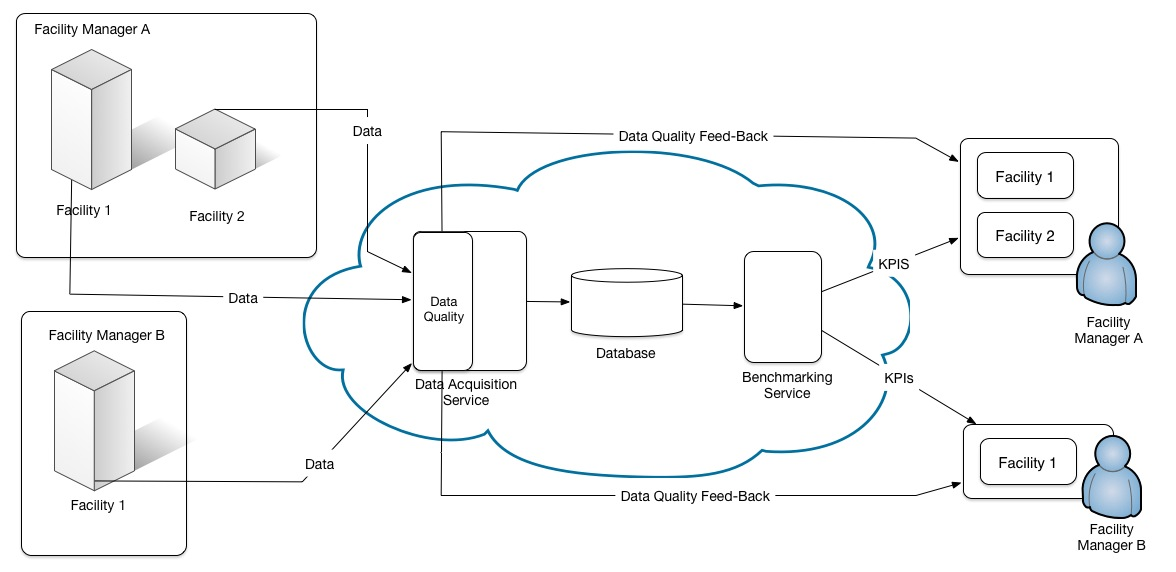
\includegraphics[width=1\textwidth]{images/OrganizacaoGeral.jpg}
  \label{fig:architecture}
\end{figure}

\end{frame}
\note[itemize]{
\item {\bf Client Side:}
\item	
			\item Running on the browser of the user connecting to the website
			\item
			\item Bootstrap Framework
			\item
			\item Javascript library highcharts or D3.js
\item
\item {\bf Server Side:}
\item
				\item Will be running the application 
				\item
				\item Will be the responsible for the processing and storage of the data sent by the Organization to the DB
				\item
				\item Play Framework
}

\begin{frame}{Architecture}

	\begin{block}{Database}
			\begin{itemize}
				\item Relational Database
				\item Theoretically divided in three
			\end{itemize}
	\end{block}


\begin{figure}
  \centering
  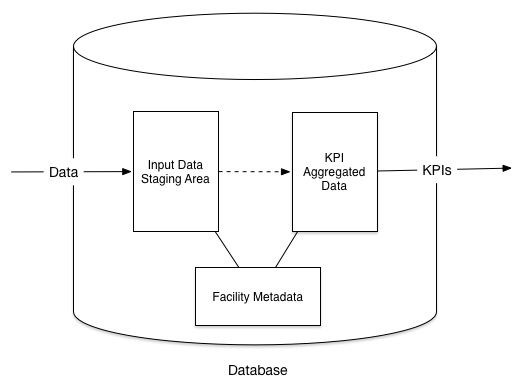
\includegraphics[width=0.60\textwidth]{images/DataBase.jpg}
  \label{fig:db}
\end{figure}

\end{frame}
\note[itemize]{
\item la
\begin{figure}
  \centering
  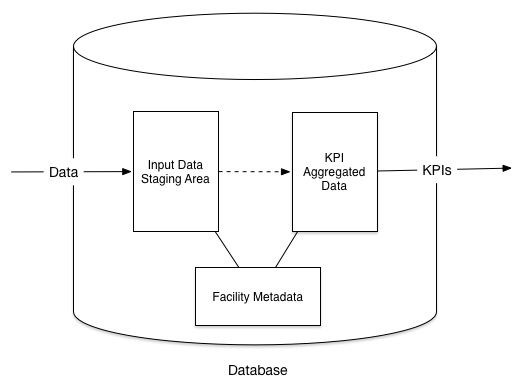
\includegraphics[width=0.60\textwidth]{images/DataBase.jpg}
  \label{fig:db}
\end{figure}
}

\begin{frame}{Deployment}

\begin{figure}
  \centering
  
\includegraphics[width=0.7\textwidth]{images/heroku.jpg}
  \label{fig:PlaneamentoTese}
\end{figure}

\end{frame}
\note[itemize]{
\item Heroku is a cloud platform as a service (PaaS) supporting several programming languages. Heroku was acquired by Salesforce.com in 2010.[1] Heroku, one of the first cloud platforms, has been in development since June 2007, when it supported only the Ruby programming language, but has since added support for Java, Node.js, Scala, Clojure, Python and PHP and (undocumented) Perl. The base operating system is Debian or, in the newest stack, the Debian-based Ubuntu.[2]
}